\documentclass[11pt,compress]{beamer}
% deactivate beamer navigation
%\setbeamertemplate{navigation symbols}{}
%\usepackage{geometry}
%\geometry{papersize={180mm, 135mm}, top=-1.5mm} % 210mm, 297mm
\usepackage{../style/lmu-lecture}
\setbeamertemplate{frametitle}{\expandafter\uppercase\expandafter\insertframetitle}

\usepackage{tikz}

\usepackage{setspace}



\AtBeginSection[]
{
  \begin{frame}<beamer>
    \frametitle{Introduction to Machine Learning}
   \begin{minipage}{\textwidth}
   %decrease linespacing to display all points
   \linespread{0.01}\selectfont
   \begin{spacing}{0.001}
   \begin{small}
      \tableofcontents[currentsection, subsectionstyle=hide]
    \end{small}
   \end{spacing}
\end{minipage}
  \end{frame}
}
% includepdf slides, pagecommad will set counter for framenumber
\usepackage{pdfpages}
\includepdfset{trim=0mm 0mm 0mm 0mm, pagecommand={\global\setcounter{framenumber}{\value{page}}}}
% trim=0mm 6mm 0mm 0mm, offset=0 15,
% add footer:
  \usepackage{framed, color}
\usepackage{xcolor}
%\iffalse
\setbeamertemplate{footline}[text line]{%
  \noindent\hspace*{\dimexpr-\oddsidemargin-1in\relax}%
  \colorbox{white}{
    \makebox[\dimexpr\paperwidth-2\fboxsep\relax]{
      \color{black}
      \begin{minipage}[c][4.5ex][c]{0.5\linewidth}
      \secname
      \end{minipage}
      \hfill\begin{minipage}[c][4.5ex][c]{0.5\linewidth}
      \flushright
      \insertframenumber{}~/~\inserttotalframenumber~~
        \end{minipage}
    }}%
  \hspace*{-\paperwidth}
}
%\fi


\title{
\hspace{-0.5cm}\centerline{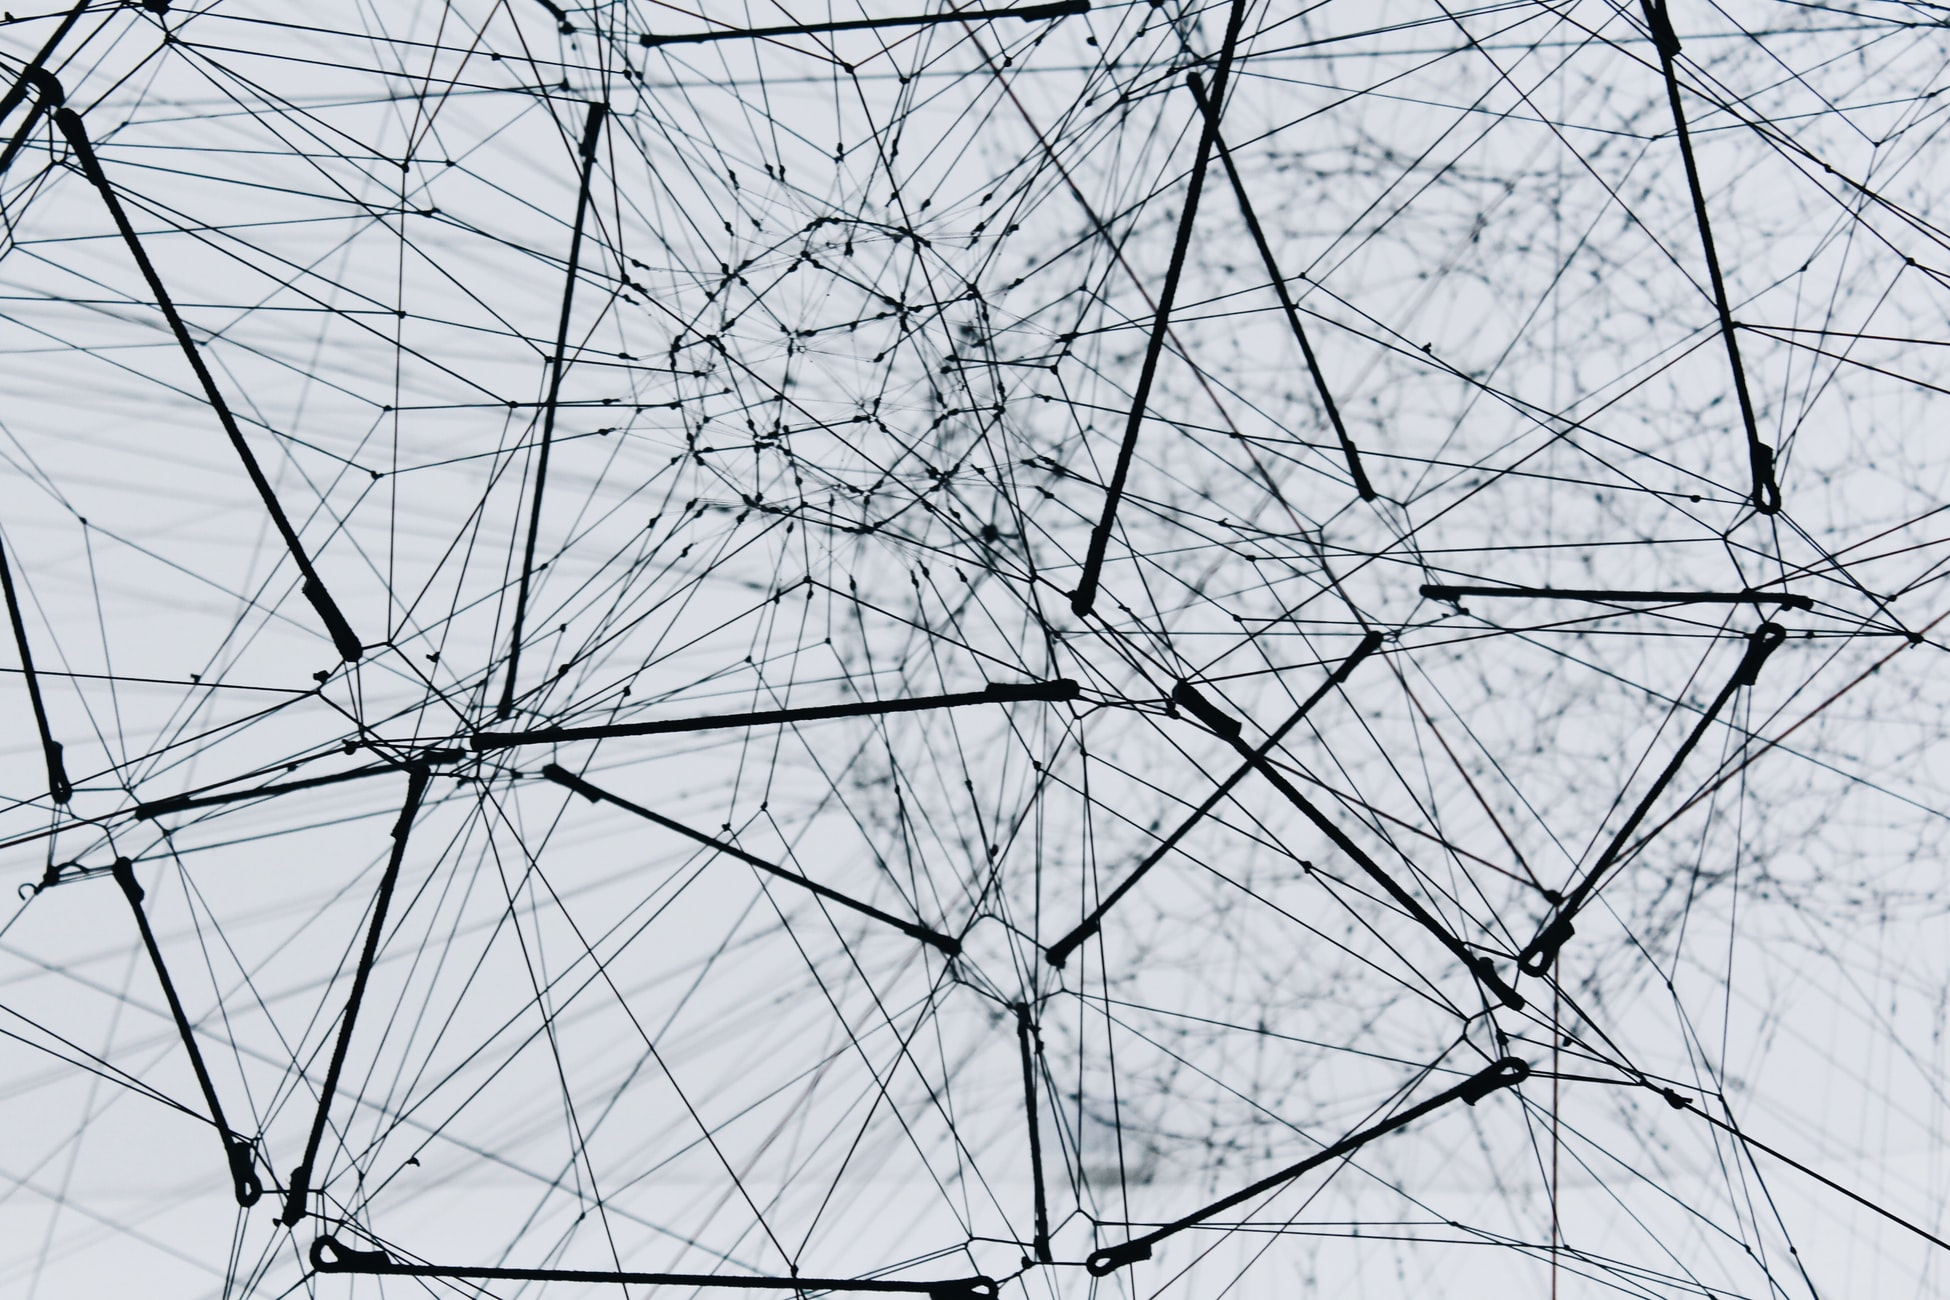
\includegraphics[width=1.05\paperwidth,keepaspectratio, trim={0 15cm 0 5cm}, clip]{titlepage.jpg}}
\medskip
Introduction to Machine Learning \\
\medskip
\small All slides
\vspace{-1.5cm}
}



\begin{document}
\setbeamercolor{background canvas}{bg=}

\begin{frame}[noframenumbering,plain]
\maketitle
\end{frame}


% General remark: hyperlinks in included pdfs are not clickable anymore in the combined pdf

% Include tuning lecture slides
\section{ML Basics}
%Suggested order of slides:

%1 slides-basics-whatisml
%2 slides-basics-data
%3 slides-basics-task
%4 slides-basics-models-parameters
%5 slides-basics-learner
%6 slides-basics-riskminimization
%7 slides-basics-optimization
%8 slides-basics-learnercomponents-hro

%slides-basics-notation is just a glossary, superseded by cheatsheet.

\subsection{What is Machine Learning?}
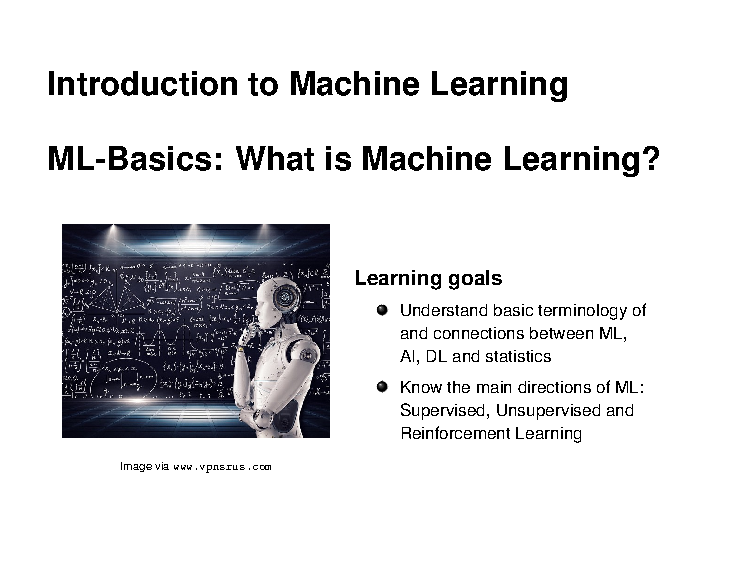
\includepdf[pages=-]{../slides-pdf/slides-basics-whatisml.pdf}

\subsection{Data}
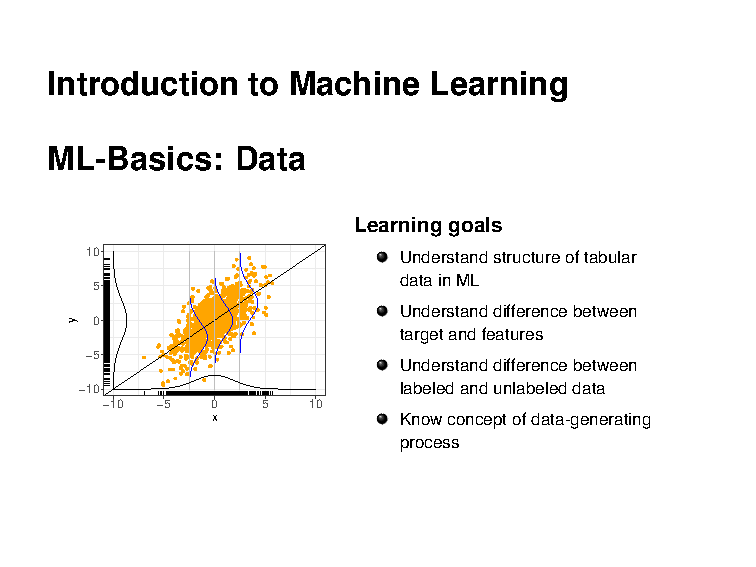
\includepdf[pages=-]{../slides-pdf/slides-basics-data.pdf}

\subsection{Supervised Tasks}
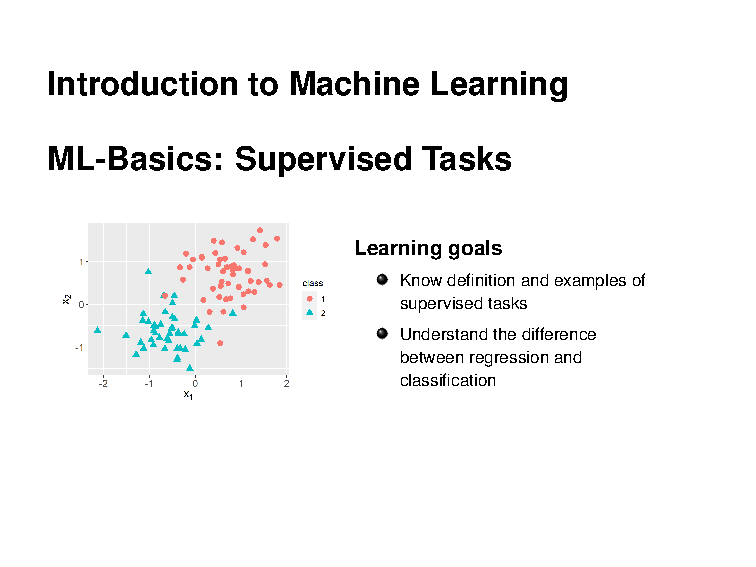
\includepdf[pages=-]{../slides-pdf/slides-basics-task.pdf}

\subsection{Models and Parameters}
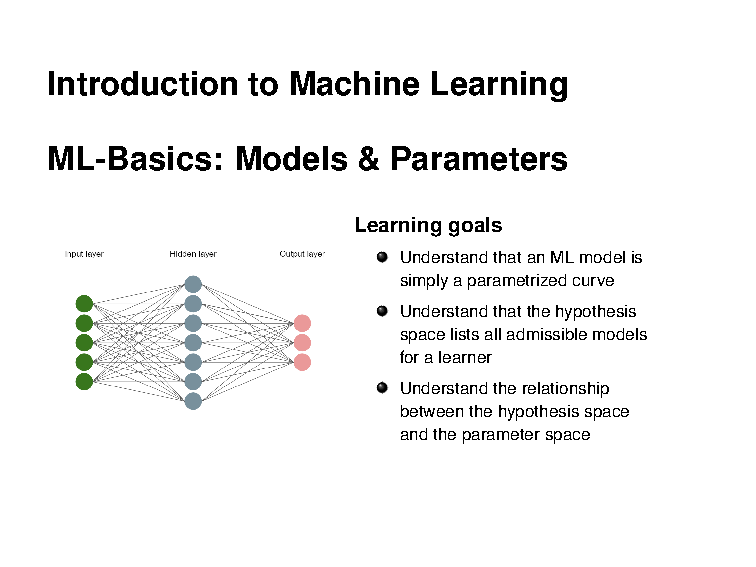
\includepdf[pages=-]{../slides-pdf/slides-basics-models-parameters.pdf}

\subsection{Learner}
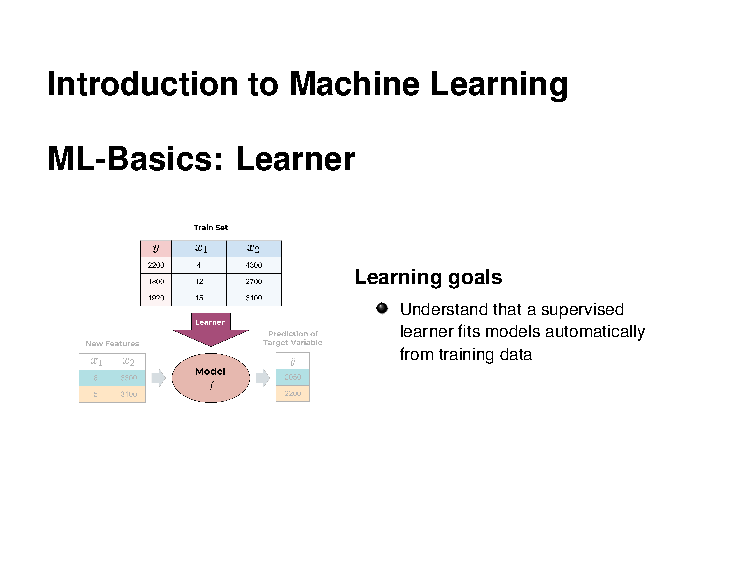
\includepdf[pages=-]{../slides-pdf/slides-basics-learner.pdf}

\subsection{Losses and Risk Minimization}
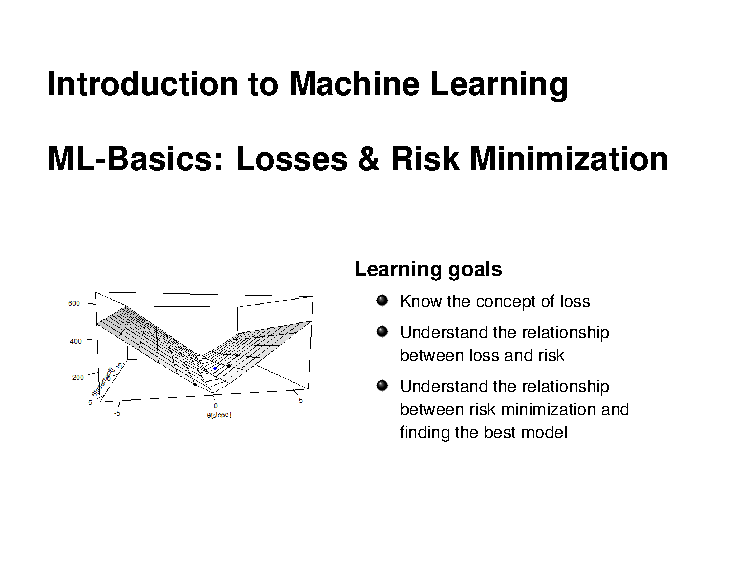
\includepdf[pages=-]{../slides-pdf/slides-basics-riskminimization.pdf}

\subsection{Optimization}
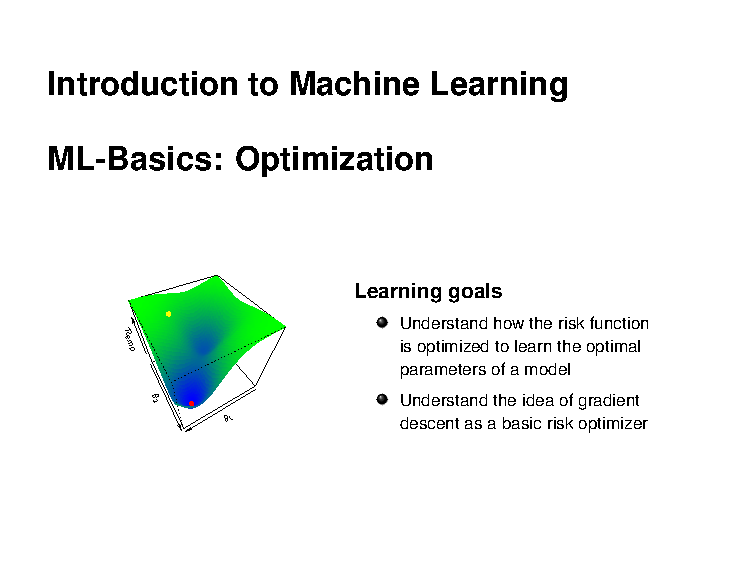
\includepdf[pages=-]{../slides-pdf/slides-basics-optimization.pdf}

\subsection{Components of Supervised Learning}
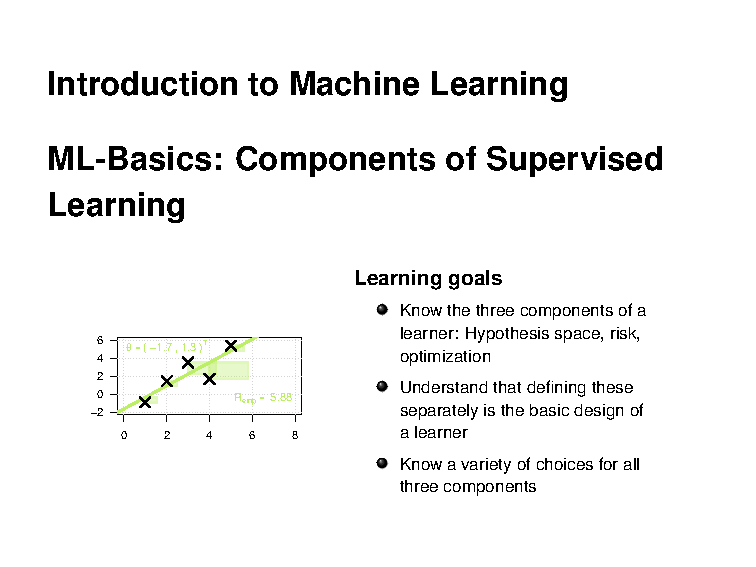
\includepdf[pages=-]{../slides-pdf/slides-basics-learnercomponents-hro.pdf}



\section{Supervised Regression}
%Suggested order of slides:

%1 slides-regression-losses
%2 slides-regression-linearmodel
%3 slides-regression-polynomials

\subsection{Loss Functions for Regression}
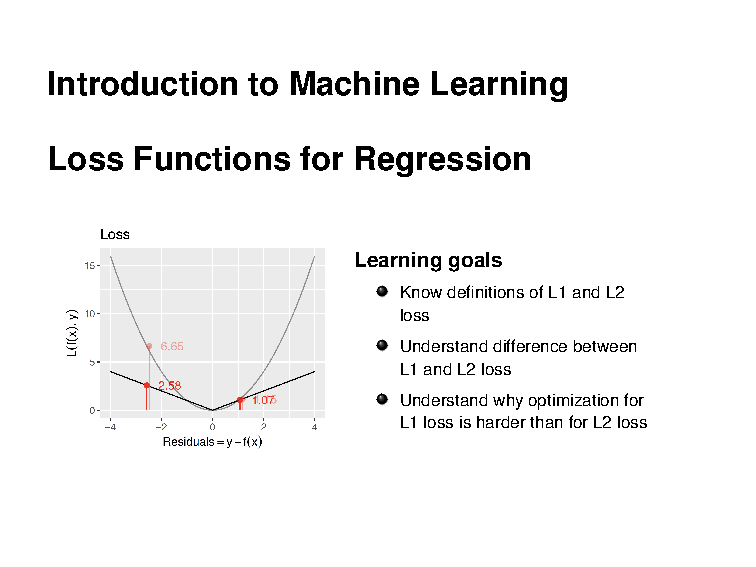
\includepdf[pages=-]{../slides-pdf/slides-regression-losses.pdf}

\subsection{Linear Regression Models}
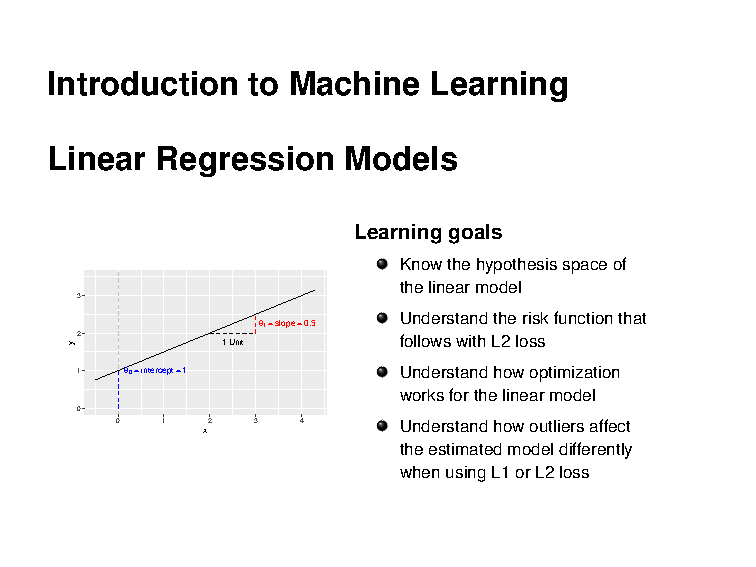
\includepdf[pages=-]{../slides-pdf/slides-regression-linearmodel.pdf}

\subsection{Polynomial Regression Models}
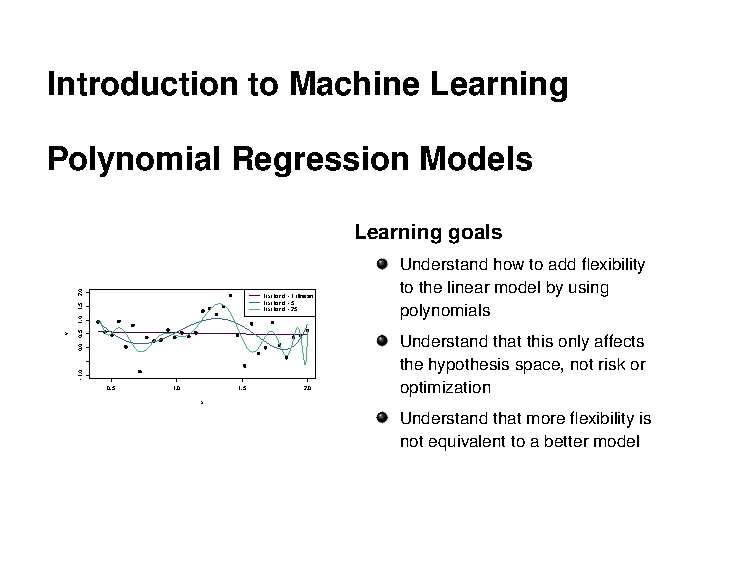
\includepdf[pages=-]{../slides-pdf/slides-regression-polynomials.pdf}

\section{Supervised Classification}
%Suggested order of slides:

%- slides-classification-tasks
%- slides-classification-basicdefs
%- slides-classification-linear
%- slides-classification-logistic
%- slides-classification-discranalysis
%- slides-classification-naivebayes

\subsection{Classification Tasks}
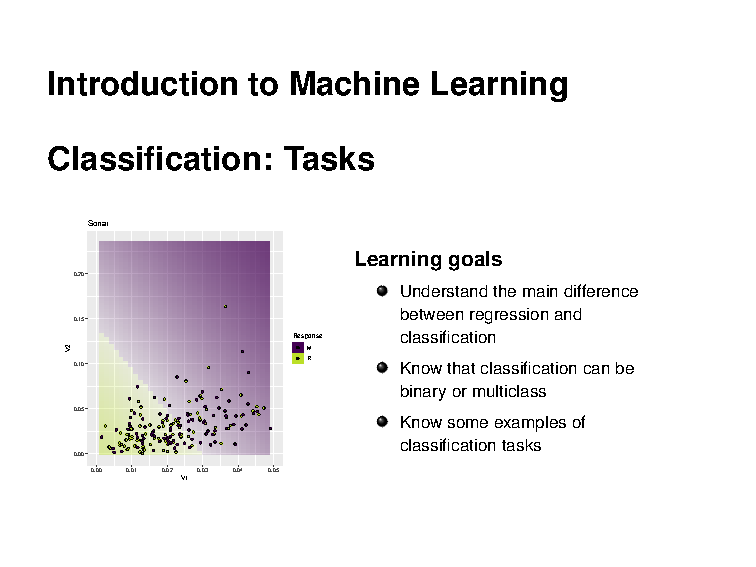
\includepdf[pages=-]{../slides-pdf/slides-classification-tasks.pdf}

\subsection{Basic Definitions}
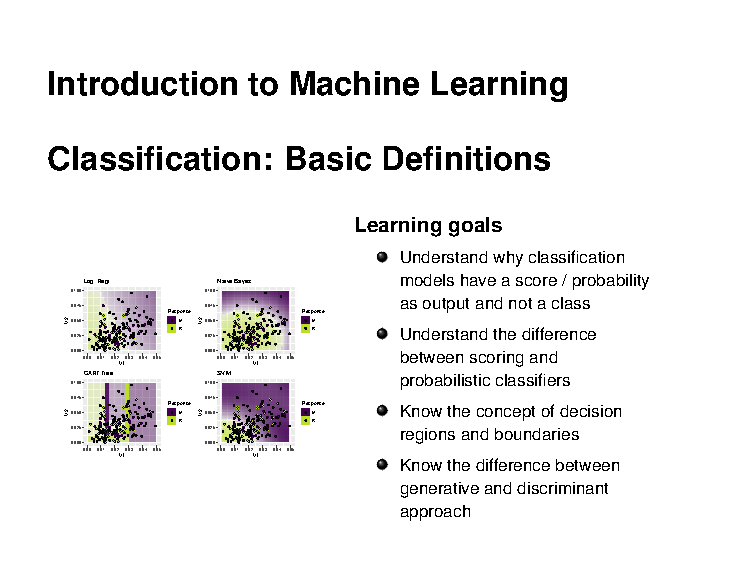
\includepdf[pages=-]{../slides-pdf/slides-classification-basicdefs.pdf}

\subsection{Linear Classifiers}
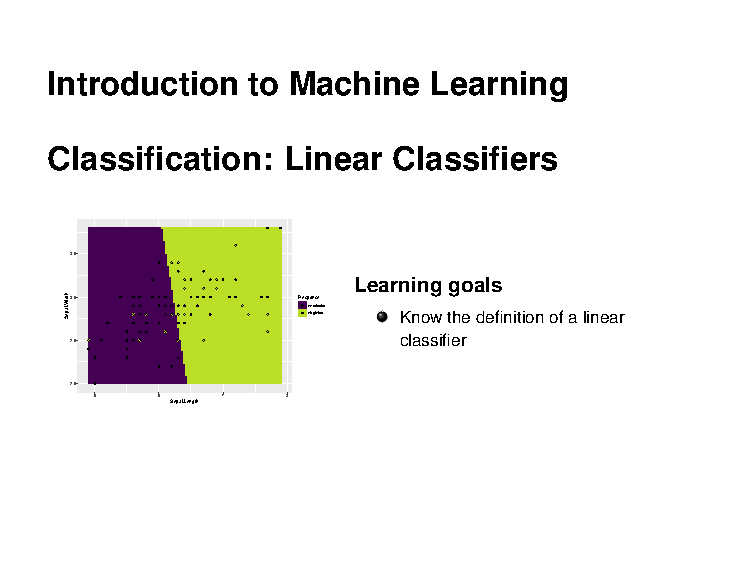
\includepdf[pages=-]{../slides-pdf/slides-classification-linear.pdf}

\subsection{Logistic Regression}
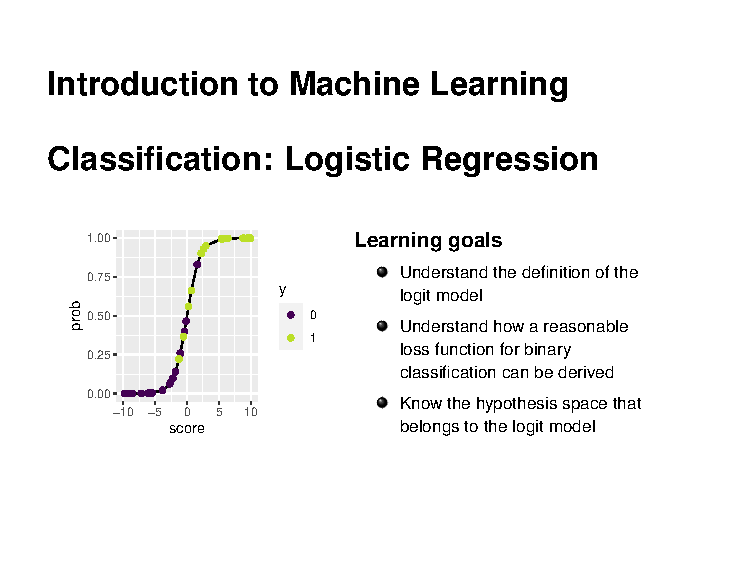
\includepdf[pages=-]{../slides-pdf/slides-classification-logistic.pdf}

\subsection{Discriminant Analysis}
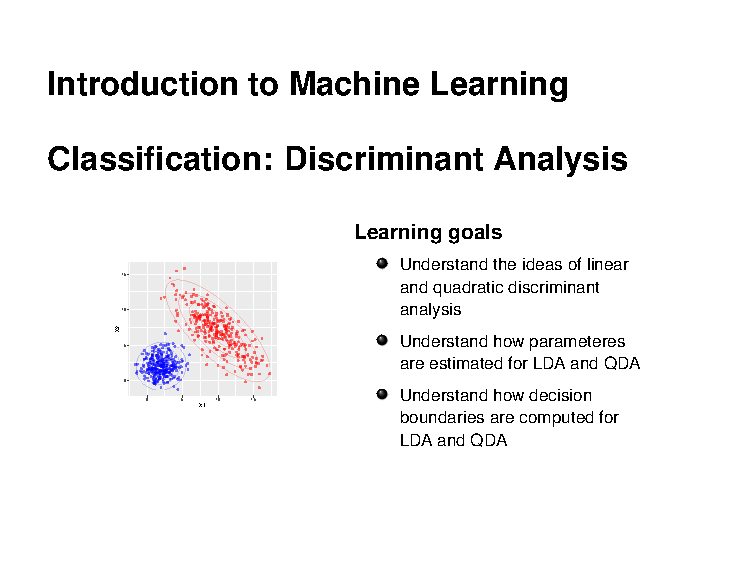
\includepdf[pages=-]{../slides-pdf/slides-classification-discranalysis.pdf}

\subsection{Naive Bayes}
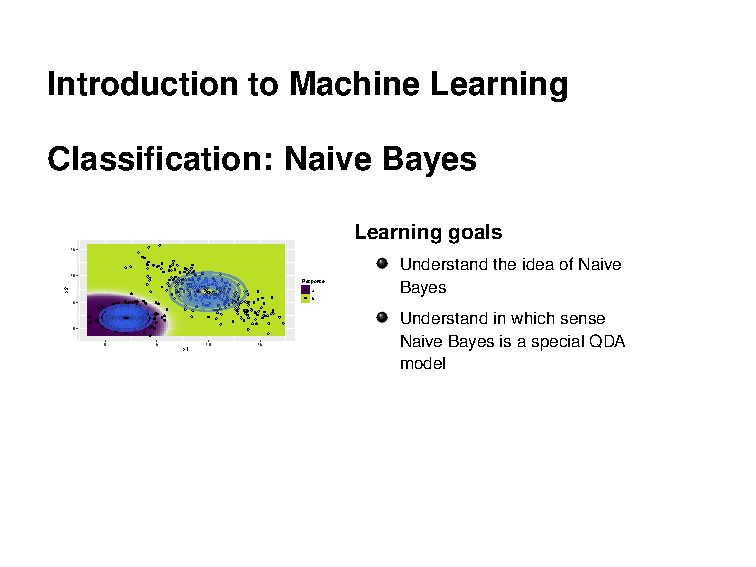
\includepdf[pages=-]{../slides-pdf/slides-classification-naivebayes.pdf}


\section{Performance Evaluation}
%Suggested order of slides:

%- slides-evaluation-intro
%- slides-evaluation-measures-regression
%- slides-evaluation-measures-classification
%- slides-evaluation-measures-classification-roc
%- slides-evaluation-measures-classification-roc-space
%- slides-evaluation-overfitting
%- slides-evaluation-train
%- slides-evaluation-test
%- slides-evaluation-resampling

\subsection{Introduction}
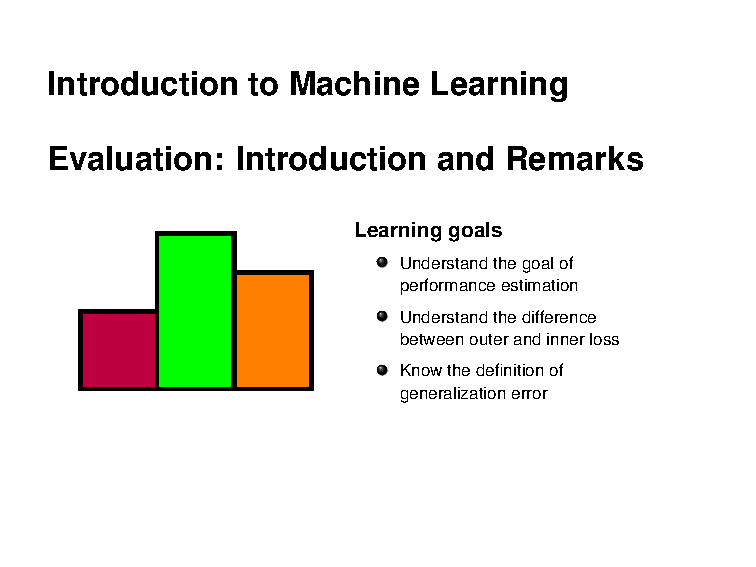
\includepdf[pages=-]{../slides-pdf/slides-evaluation-intro.pdf}

\subsection{Measures Regression}
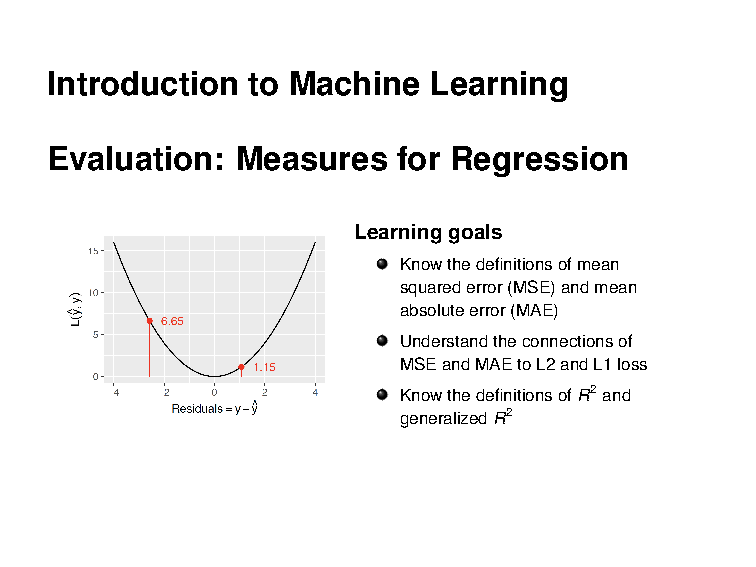
\includepdf[pages=-]{../slides-pdf/slides-evaluation-measures-regression.pdf}

\subsection{Measures Classification}
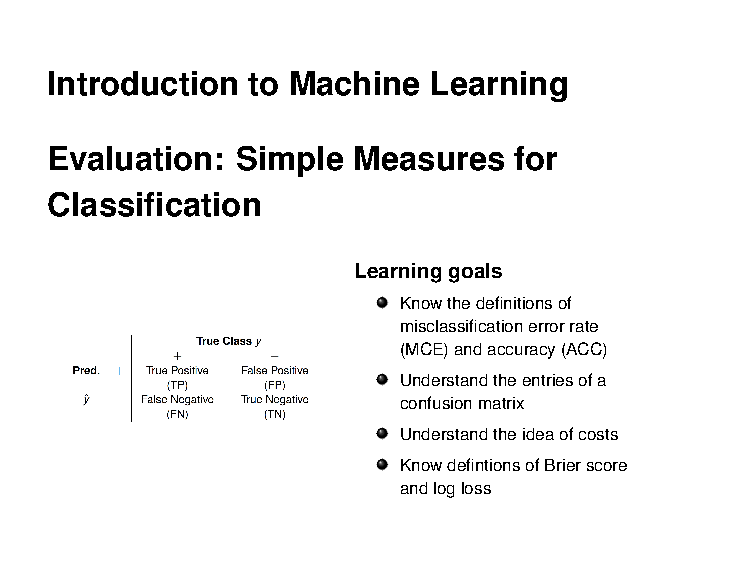
\includepdf[pages=-]{../slides-pdf/slides-evaluation-measures-classification.pdf}

\subsection{Measures Classification ROC}
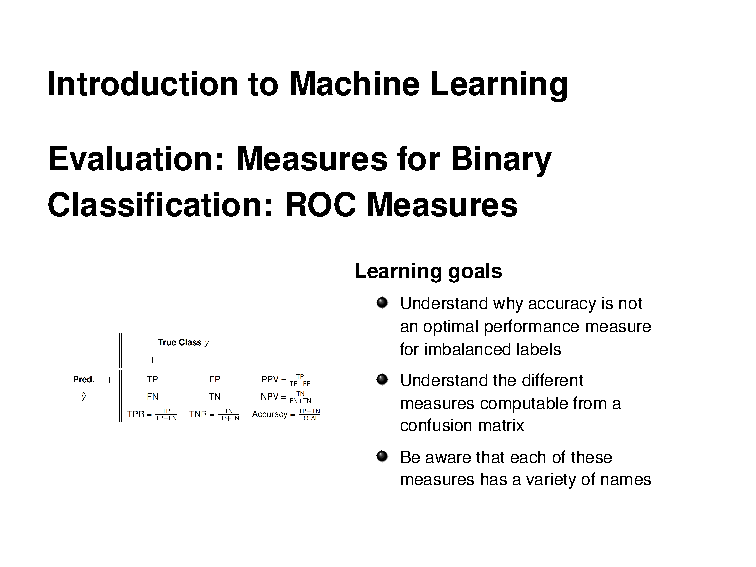
\includepdf[pages=-]{../slides-pdf/slides-evaluation-measures-classification-roc.pdf}

\subsection{Measures Classification ROC Visualisation}
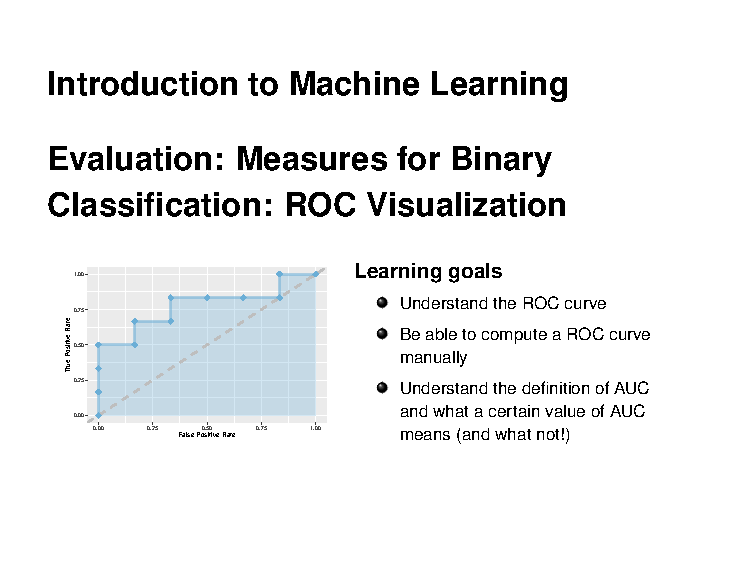
\includepdf[pages=-]{../slides-pdf/slides-evaluation-measures-classification-roc-space.pdf}

\subsection{Overfitting}
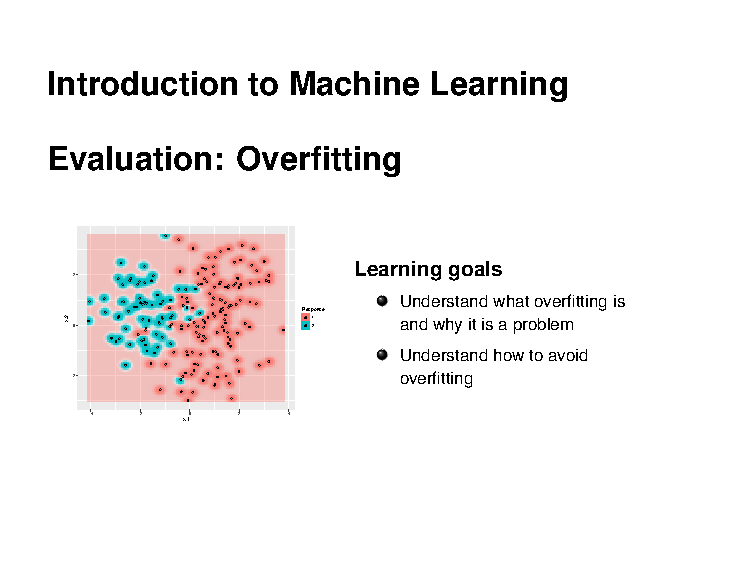
\includepdf[pages=-]{../slides-pdf/slides-evaluation-overfitting.pdf}

\subsection{Training Error}
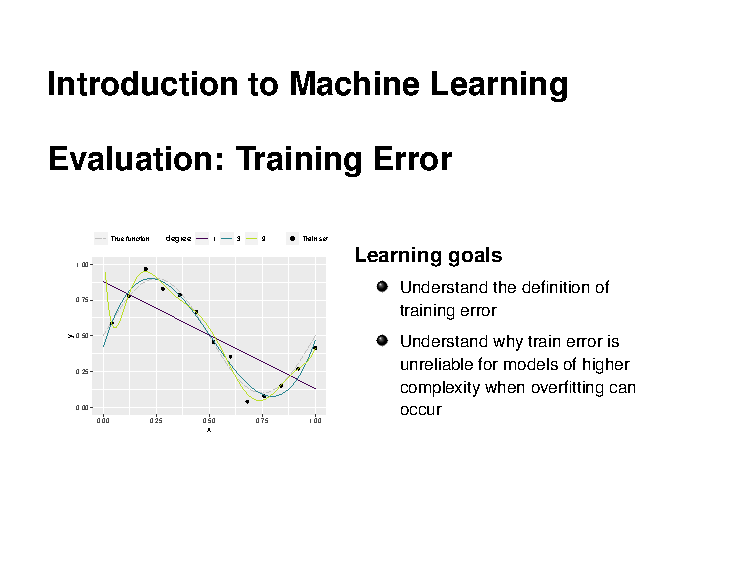
\includepdf[pages=-]{../slides-pdf/slides-evaluation-train.pdf}

\subsection{Test Error}
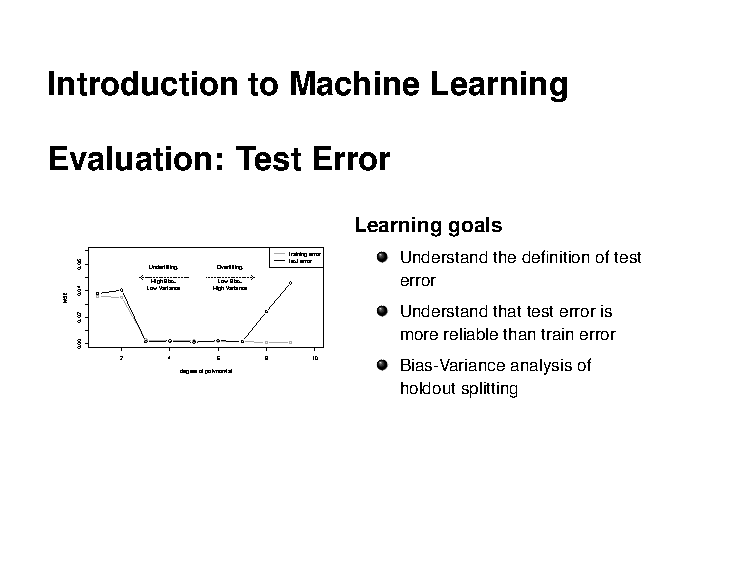
\includepdf[pages=-]{../slides-pdf/slides-evaluation-test.pdf}

\subsection{Resampling}
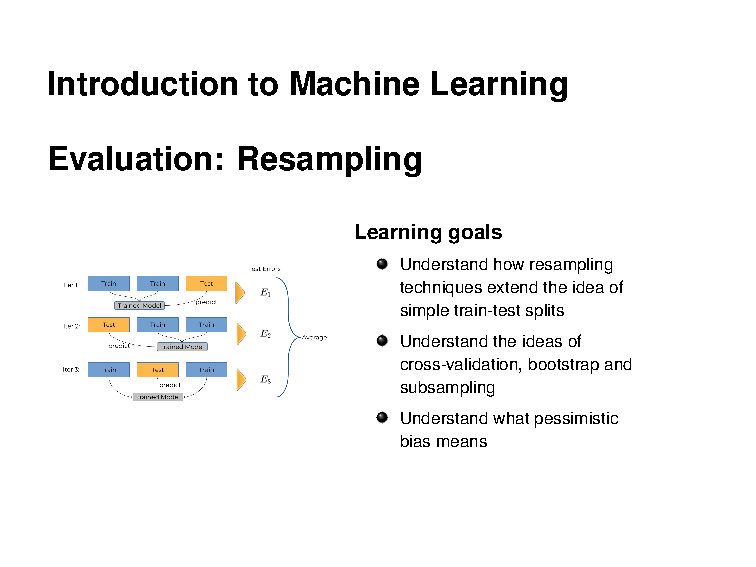
\includepdf[pages=-]{../slides-pdf/slides-evaluation-resampling.pdf}


\section{k-NN}
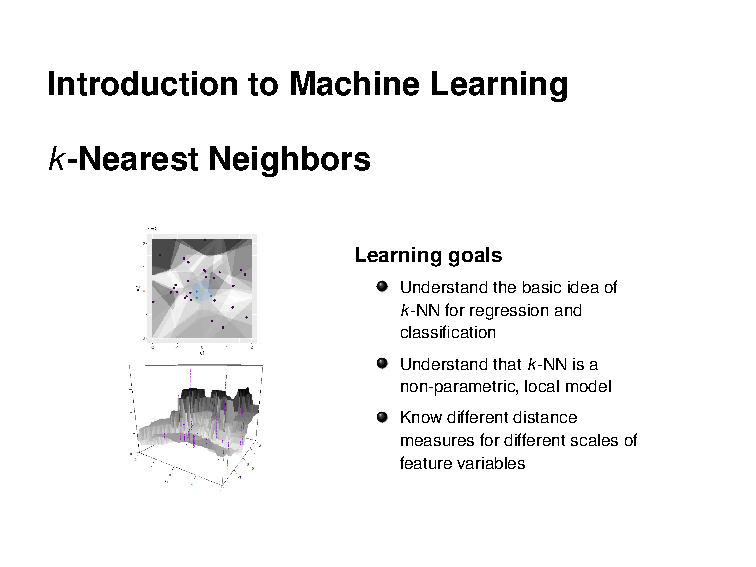
\includepdf[pages=-]{../slides-pdf/slides-knn.pdf}

\section{Classification and Regression Trees (CART)}
%Suggested order of slides:

%1 slides-cart-intro
%2 slides-cart-splitcriteria
%3 slides-cart-treegrowing
%4 slides-cart-splitcomputation
%5 slides-cart-stoppingpruning
%6 slides-cart-discussion

\subsection{Introduction}
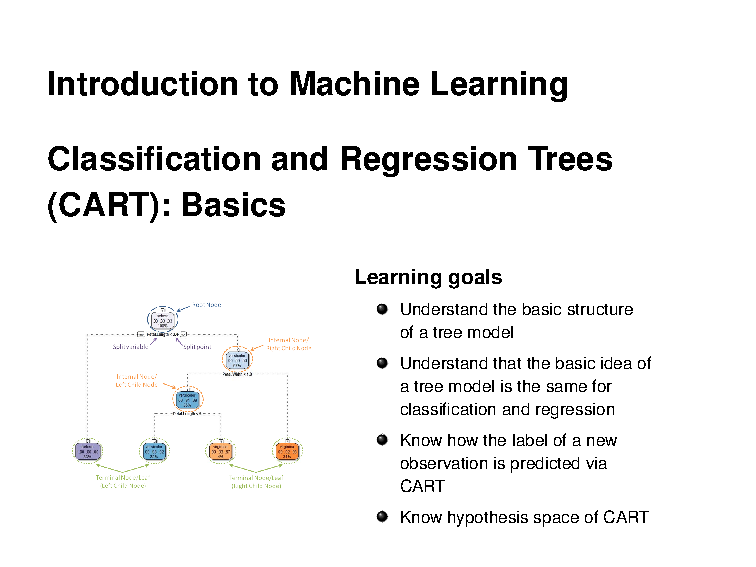
\includepdf[pages=-]{../slides-pdf/slides-cart-intro.pdf}

\subsection{Splitting Criteria}
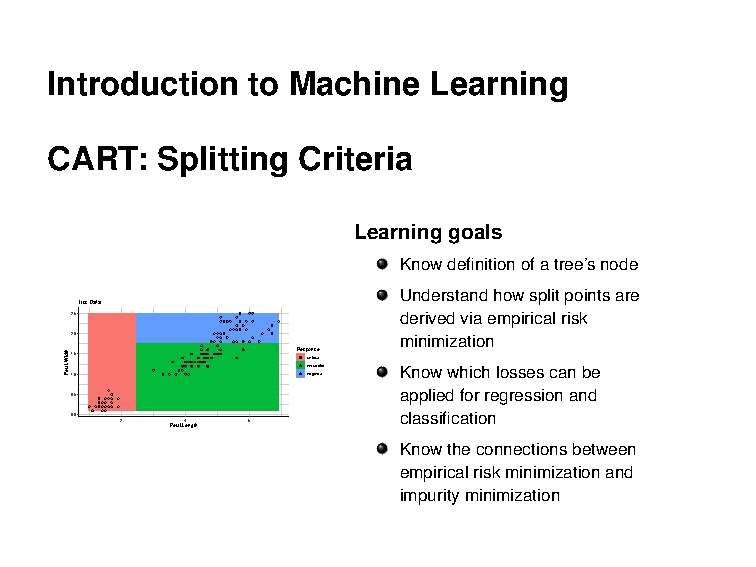
\includepdf[pages=-]{../slides-pdf/slides-cart-splitcriteria.pdf}

\subsection{Growing a Tree}
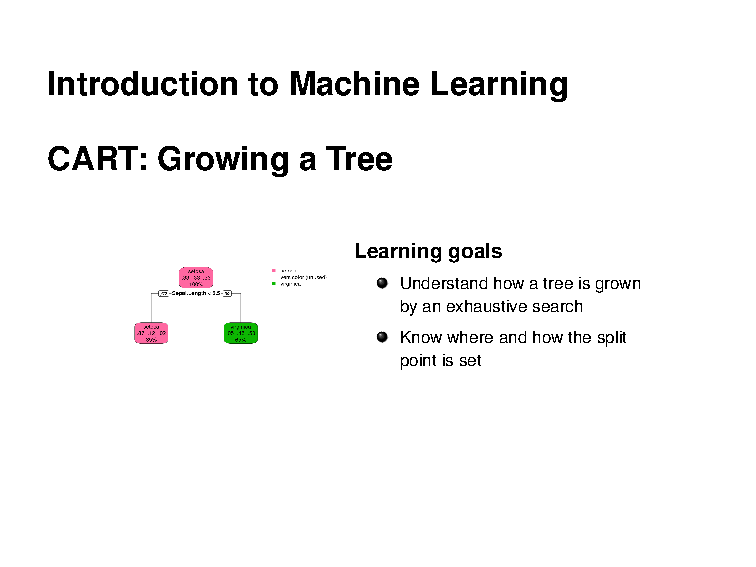
\includepdf[pages=-]{../slides-pdf/slides-cart-treegrowing.pdf}

\subsection{Computational Aspects of Finding Splits}
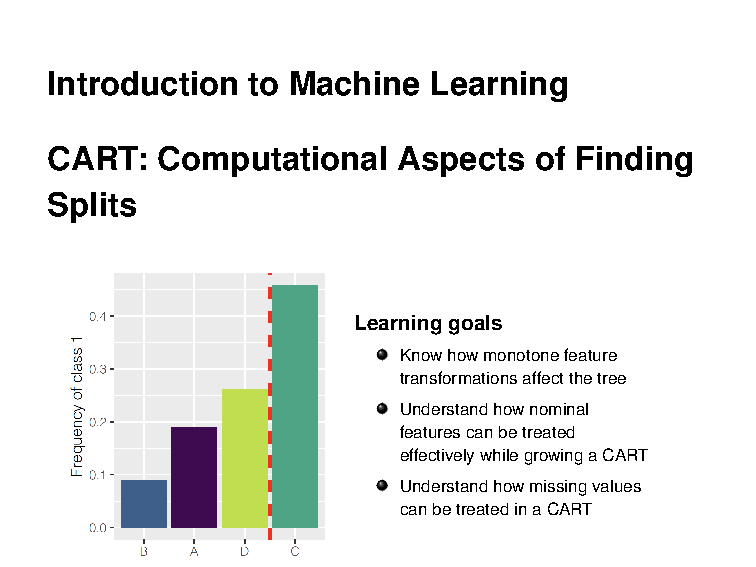
\includepdf[pages=-]{../slides-pdf/slides-cart-splitcomputation.pdf}

\subsection{Stopping criteria \& pruning}
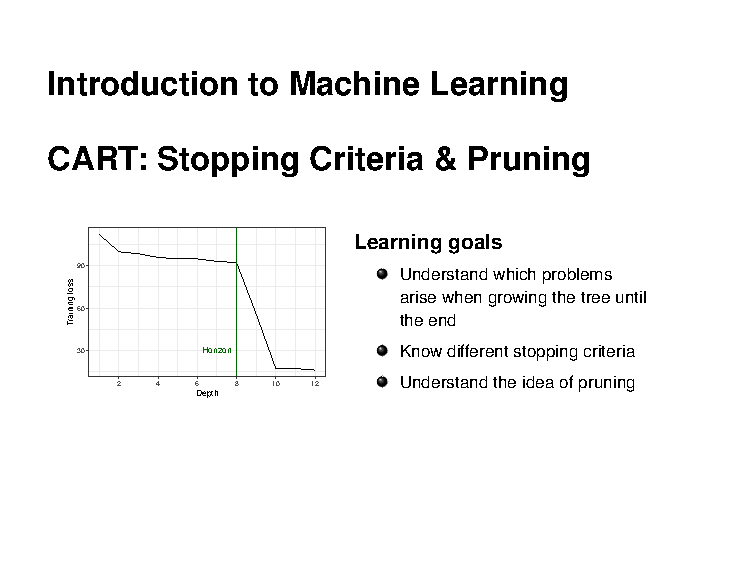
\includepdf[pages=-]{../slides-pdf/slides-cart-stoppingpruning.pdf}

\subsection{Discussion}
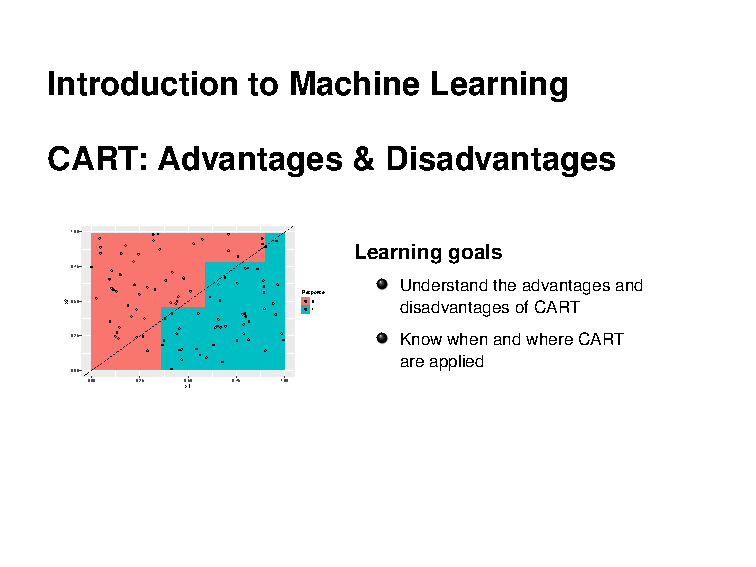
\includepdf[pages=-]{../slides-pdf/slides-cart-discussion.pdf}


\section{Random Forests}
%Suggested order of slides:

%1 slides-forests-bagging
%2 slides-forests-intro
%3 slides-forests-benchmark
%4 slides-forests-featureimportance
%5 slides-forests-proximities
%6 slides-forests-discussion

\subsection{Bagging Ensembles}
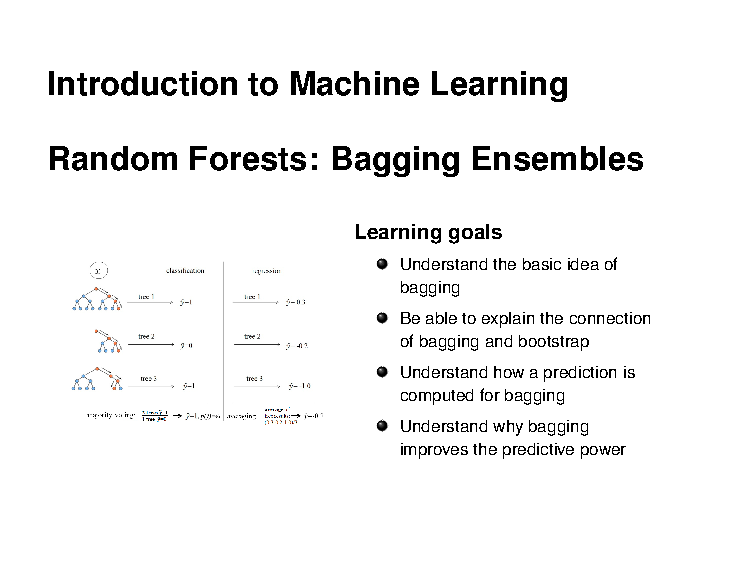
\includepdf[pages=-]{../slides-pdf/slides-forests-bagging.pdf}

\subsection{Introduction}
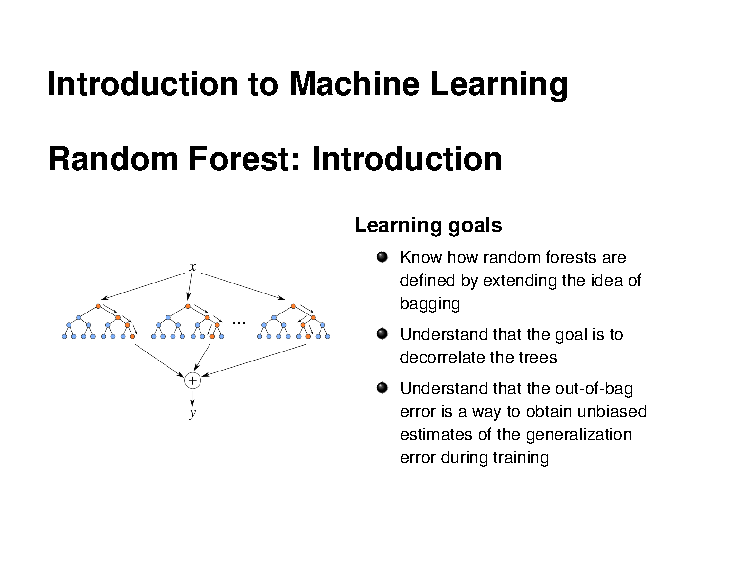
\includepdf[pages=-]{../slides-pdf/slides-forests-intro.pdf}

\subsection{Benchmarking Trees, Forests, and Bagging K-NN}
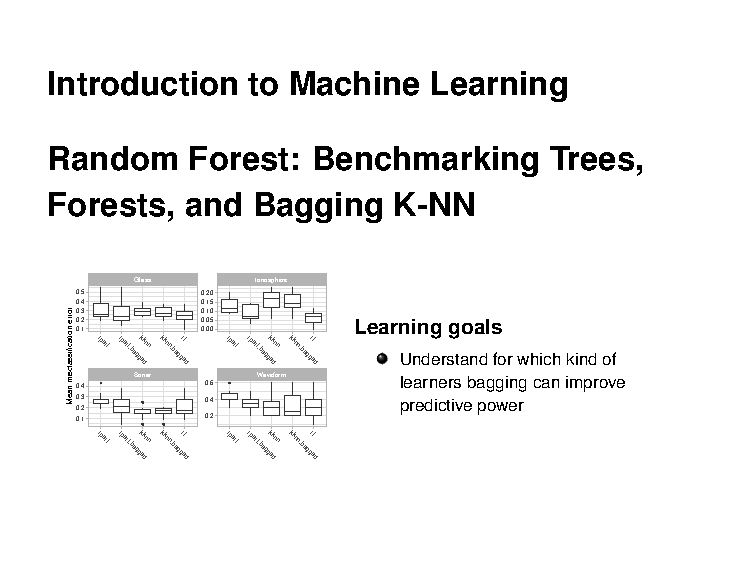
\includepdf[pages=-]{../slides-pdf/slides-forests-benchmark.pdf}

\subsection{Feature Importance}
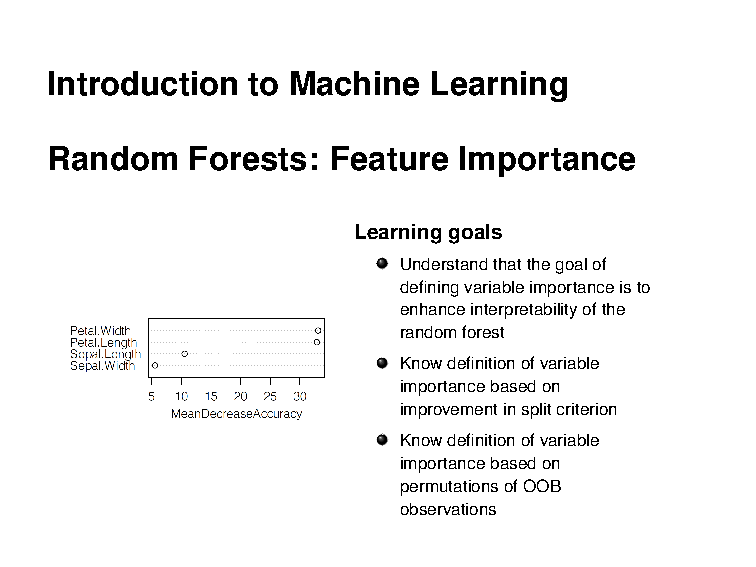
\includepdf[pages=-]{../slides-pdf/slides-forests-featureimportance.pdf}

\subsection{Proximities}
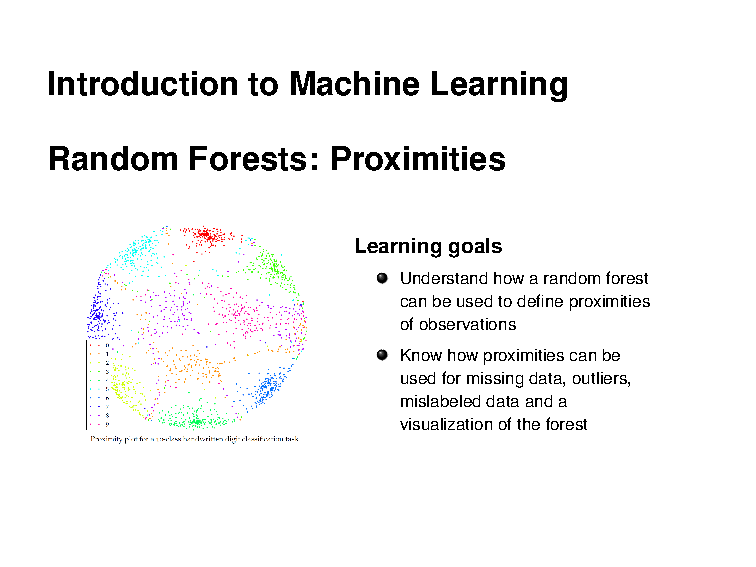
\includepdf[pages=-]{../slides-pdf/slides-forests-proximities.pdf}

\subsection{Discussion}
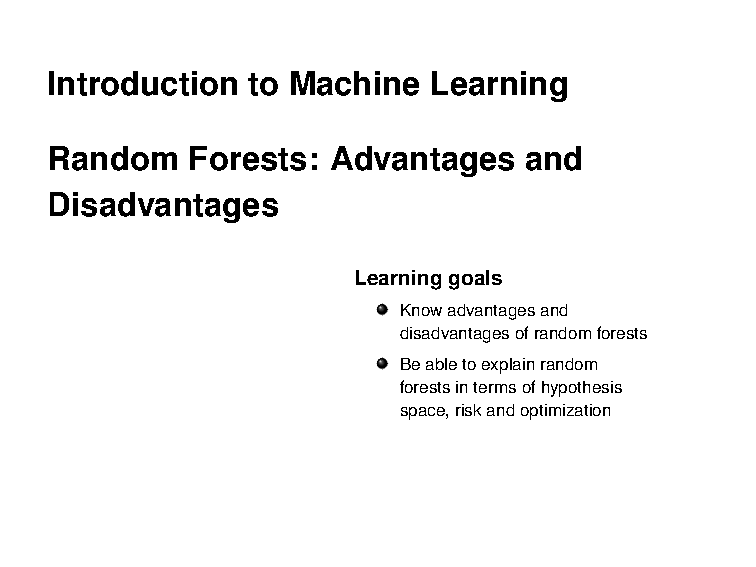
\includepdf[pages=-]{../slides-pdf/slides-forests-discussion.pdf}

\section{Tuning}
%Suggested order of slides:

%- slides-tuning-intro
%- slides-tuning-tuningproblem
%- slides-tuning-basicalgos
%- slides-tuning-advanced
%- slides-tuning-pipelines
%- slides-tuning-practical

\subsection{Introduction}
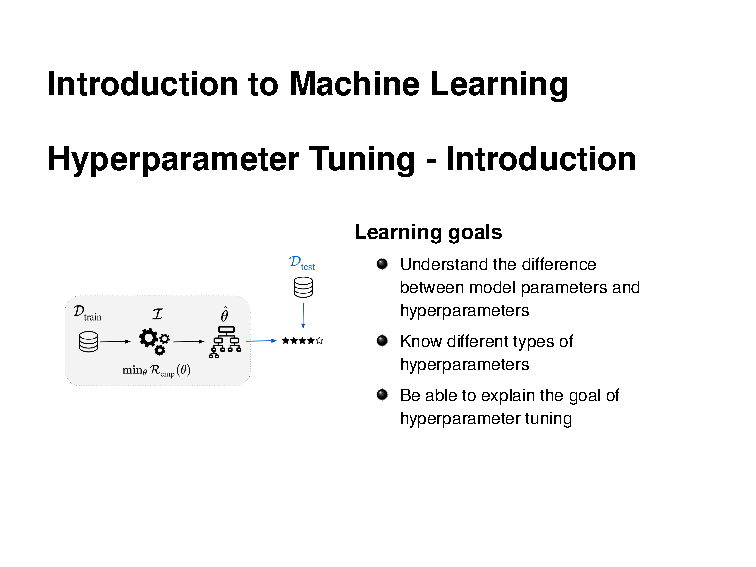
\includepdf[pages=-]{../slides-pdf/slides-tuning-intro.pdf}

\subsection{Problem Definition}
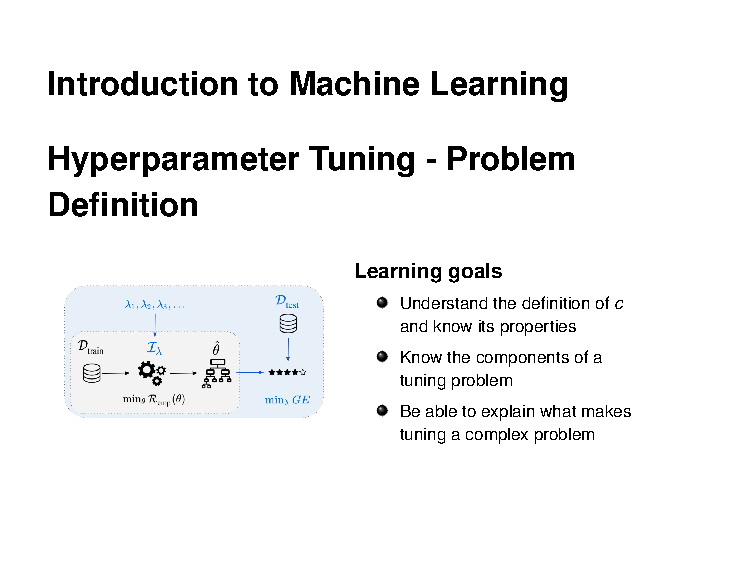
\includepdf[pages=-]{../slides-pdf/slides-tuning-tuningproblem.pdf}

\subsection{Basic Techniques}
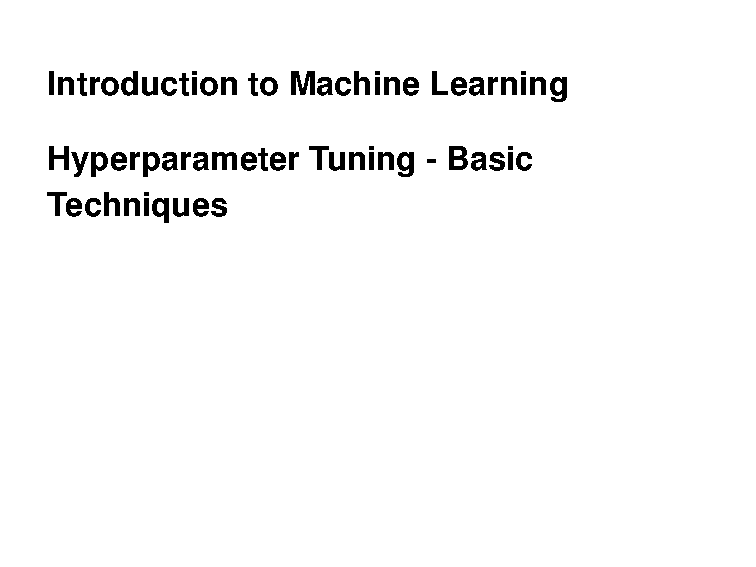
\includepdf[pages=-]{../slides-pdf/slides-tuning-basicalgos.pdf}

\subsection{Advanced Techniques}
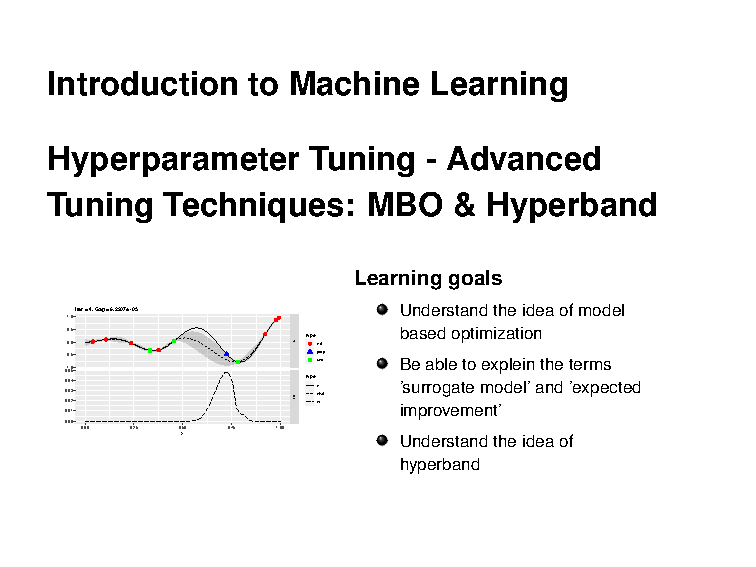
\includepdf[pages=-]{../slides-pdf/slides-tuning-advanced.pdf}

\subsection{Pipelines and AutoML}
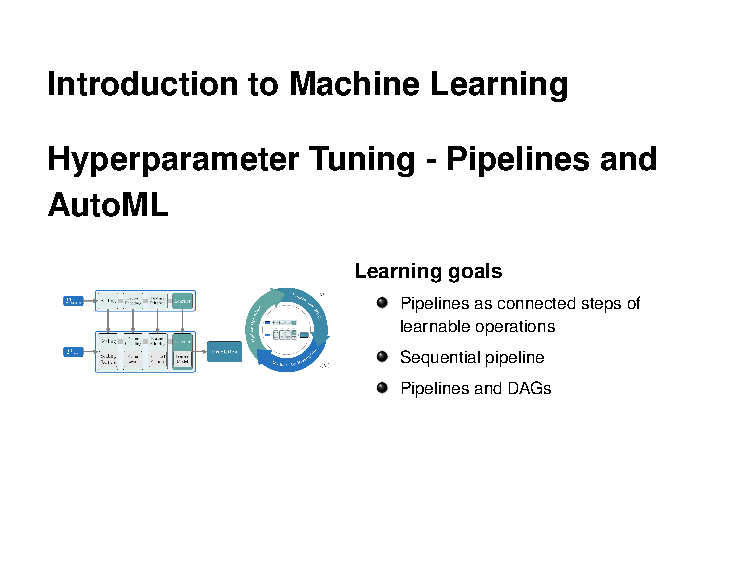
\includepdf[pages=-]{../slides-pdf/slides-tuning-pipelines.tex}

\subsection{Practical Aspects}
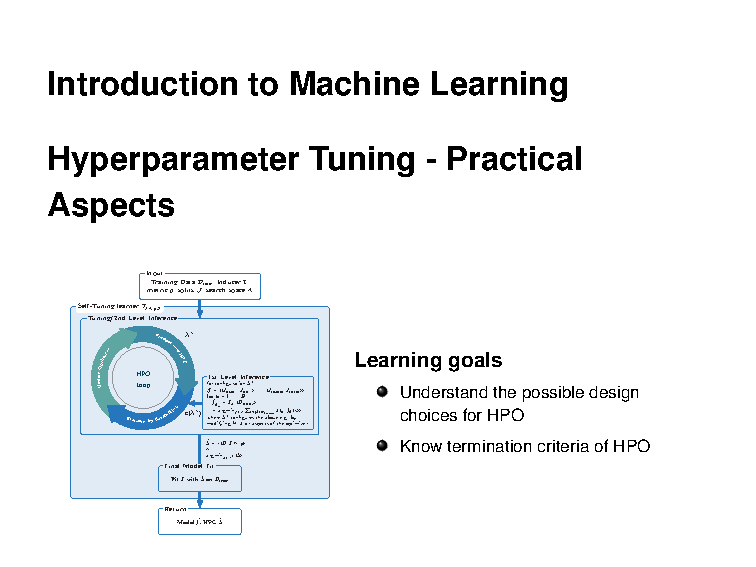
\includepdf[pages=-]{../slides-pdf/slides-tuning-practical.pdf}


\section{Nested Resampling}
%Suggested order of slides:

%- slides-nested-nestedintro
%- slides-nested-trainvalidtest
%- slides-nested-nestedresampling

\subsection{Motivation}
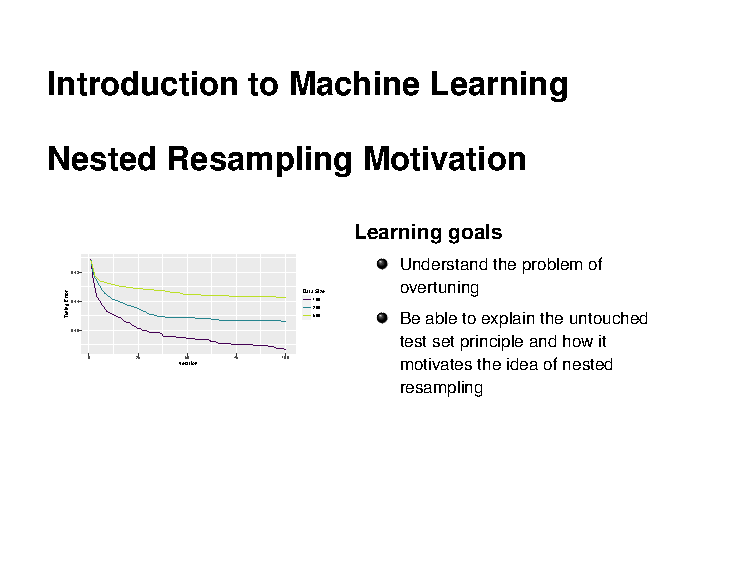
\includepdf[pages=-]{../../slides-pdf/slides-nested-nestedintro.pdf}

\subsection{Training - Validation - Testing}
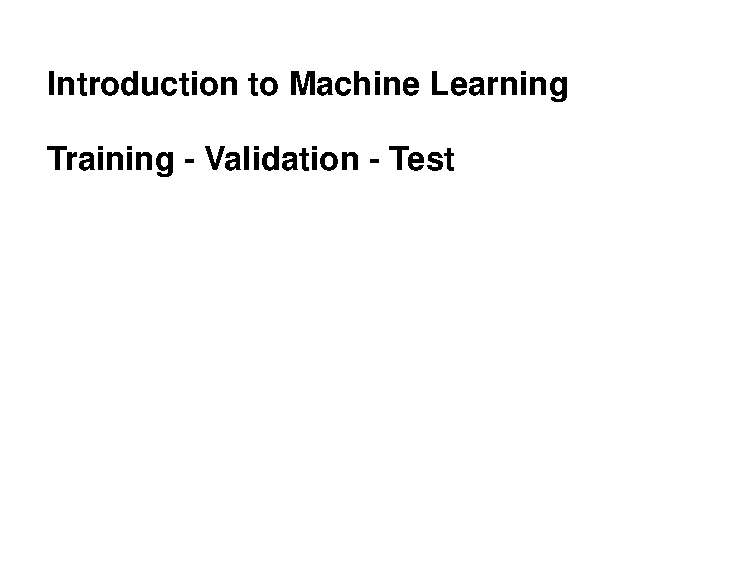
\includepdf[pages=-]{../../slides-pdf/slides-nested-trainvalidtest.pdf}

\subsection{Nested Resampling}
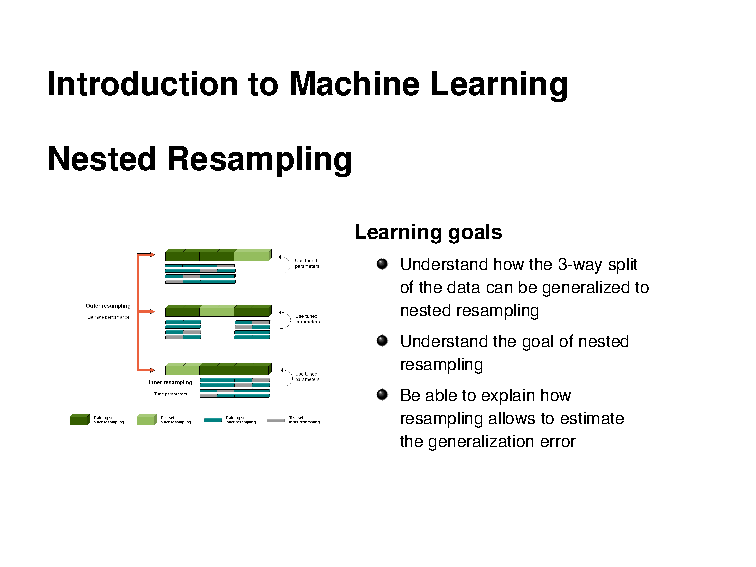
\includepdf[pages=-]{../../slides-pdf/slides-nested-nestedresampling.pdf}



\section{mlr3}
%Suggested order of slides:
\subsection{Intro to mlr3}
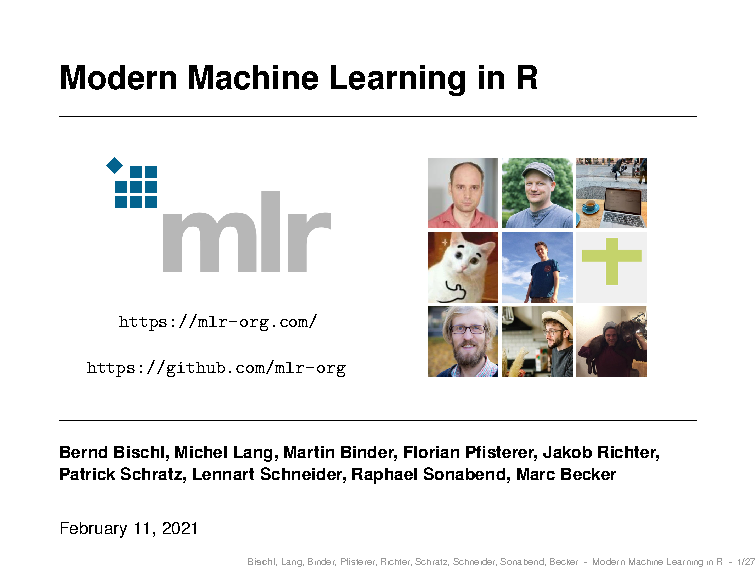
\includepdf[pages=-]{../../slides-pdf/slides-mlr3-intro.pdf}

\subsection{Resampling with mlr3}
\includepdf[pages=-]{../../slides-pdf/slides-mlr3-resampling.pdf}

\subsection{Tuning with mlr3}
\includepdf[pages=-]{../../slides-pdf/slides-mlr3-tuning.pdf}

\subsection{Pipelines with mlr3}
\includepdf[pages=-]{../../slides-pdf/slides-mlr3-pipelines.pdf}



\end{document}
  